\documentclass[preprint]{sigplanconf}
\usepackage{xspace,listings,url,subfigure,framed,amssymb,
            amsmath,mathpartir,hyperref,
            stmaryrd, graphicx % double brackets llbracket
}
\newcommand{\rn}[1]{#1}
\newcommand{\doi}[1]{doi:~\href{http://dx.doi.org/#1}{\Hurl{#1}}}

\conferenceinfo{CONF 'yy}{Month d--d, 20yy, City, ST, Country}
\copyrightyear{20yy}
\copyrightdata{978-1-nnnn-nnnn-n/yy/mm}
\copyrightdoi{nnnnnnn.nnnnnnn}

%%% Metavariables %%%%%%%%%%%%%%%%%%%
\newcommand{\fd}{\M{\xt{fd}}}
\newcommand{\md}{\M{\xt{md}}}
\newcommand{\mt}{\M{\xt{mt}}}
\newcommand{\m}{\M{\xt{m}}}
\newcommand{\e}{\M{\xt{e}}}
\newcommand{\n}{\M{\xt{n}}}
\renewcommand{\d}{\M{\xt{d}}}
\renewcommand{\r}{\M{\xt{r}}}
\newcommand{\f}{\M{\xt{f}}}
\newcommand{\fb}{\M{\xt{f!}}}
\newcommand{\x}{\M{\xt{x}}}
\renewcommand{\t}{\M{\xt{t}}}
\renewcommand{\c}{\M{\xt{c}}}
\newcommand{\C}{\M{\xt{C}}}
\newcommand{\D}{\M{\xt{D}}}
\newcommand{\this}{\M{\xt{this}}}
\newcommand{\err}{\M{\bt{err}}}
\renewcommand{\d}{\M{\xt{d}}}
\newcommand{\s}{\M{\sigma}}
\renewcommand{\a}{\M{\xt a}}
\newcommand{\T}{\M{\xt T}}
\newcommand{\tp}[1]{\M{ \t_{#1} }}
\newcommand{\ep}[1]{\M{ \e_{#1} }}
\newcommand{\ap}[1]{\M{ \a_{#1} }}
\renewcommand{\mp}[1]{\M{ \m_{#1} }}
\renewcommand{\sp}[1]{\M{ \s_{#1} }}
\newcommand{\none}{\M{\cdot}}
%% Keywords %%%%%%%%%%%%%%%%%%
\newcommand{\new}{\M{\bt{new}}}
\newcommand{\class}{\M{\bt{class}}}
%% Expressions %%%%%%%%%%%%%%%%%%%%
\newcommand{\Get}[2]{\M{#1.#2}}
\newcommand{\Set}[3]{\M{#1.#2:=#3}}
\newcommand{\Call}[3]{\M{#1.#2(#3)}}
\newcommand{\New}[2]{\M{\new\;#1({#2})}}
\newcommand{\Cast}[2]{\M{\langle{#1}\rangle{#2}}}
%% Types %%%%%%%%%%%%%%%%%%%%%%%%%%%
\newcommand{\any}{\M{\star}}
\newcommand{\Type}[1]{\M{\{ #1 \}}}
\newcommand{\HT}[2]{\M{{#1}\!:{#2}}}
%% Classes %%%%%%%%%%%%%%%%%%%%%%%%%
\newcommand{\Mdef}[5]{\M{ \HT { #1( \b{\HT{#2}{#3}})}{#4}~ \{\, {#5} \,\} }}
\newcommand{\SMdef}[5]{\M{ \HT { #1!( \HT{#2}{#3})}{#4}= {#5}}}
\newcommand{\GMdef}[3]{\M{ \HT { #1()}{#2}={#3}}}
\newcommand{\Ftype}[2]{\M{ \HT{#1}{#2} }}
\newcommand{\Fdef}[3]{\M{ \HT{#1}{#2}={#3} }}
\newcommand{\Mtype}[3]{\M{ \HT { #1( #2 )}{#3}}}
\newcommand{\Class}[3]{\M{\bt{class}\;#1\,\{\, #2 ~ #3\, \}}}
%%% Dynamics %%%%%%%%%%%%%%%%%%%%%%%%%
\newcommand{\is}{\M{\mapsto}}
\newcommand{\Obj}[2]{ \M{\{ #1 \B {#2}\}}}
\newcommand{\Heap}[2]{\M{ #1[ #2 ] }}
\newcommand{\alloc}[4]{\M{#1,#2  = \xt{alloc}(#3, #4)}}
\newcommand{\dispatch}[5]{\M{#1,#2 = \xt{dispatch}(#3,#4,#5)}}
\newcommand{\notdispatch}[5]{\M{#1,#2 \not = \xt{dispatch}(#3,#4,#5)}}
\newcommand{\readfield}[4]{\M{#1 = \xt{readfield}(#2,#3,#4)}}
\newcommand{\setfield}[5]{\M{#1 = \xt{writefield}(#2,#3,#4,#5)}}


%% Formatting %%%%%%%%%%%%%%%%%%%%%%%%%%%
\newcommand{\Alt}[1]{ &\B #1 \\}
\newcommand{\B}{\M{~|~}}
\newcommand{\M}[1]{\ensuremath{#1}\xspace}
\newcommand{\xt}[1]{{\sf{#1}}\xspace}
\newcommand{\bt}[1]{\xt{\bf #1}}
\renewcommand{\b}[1]{\M{\overline{#1}}}
\newcommand{\opdef}[2]{\framebox[1.1\width]{#1} ~ #2\\}

\newcommand{\IRule}[3]{\inferrule*[lab={\tiny #1}]{#2}{#3}}
%\newcommand{\IRule}[3]{\inferrule{#2}{#3}}    %% No label
\newcommand{\CondRule}[3]{ #3 &~{\emph{if}} #2 \\}
\newcommand{\NoCondRule}[2]{ #2 &       \\}
\newcommand{\Reduce}[4]{\M{ #1~#2 \rightarrow #3~#4}}
\newcommand{\ReduceA}[4]{\M{ #1 ~ #2 } &  \M { \rightarrow #3 ~ #4}}
\newcommand{\inc}{\M{\in}}
\newcommand{\Update}[3]{\M{#1[ #2 := #3]}}
\newcommand{\Bind}[2]{\M{#1 \is #2}}
\newcommand{\NotSub}{\M{\not<:}}
\newcommand{\Sub}{\M{<:}}
\newcommand{\classofis}[2]{\M{\xt{classof}(#1)=#2}}
\newcommand{\typeofis}[3]{\M{\xt{typeof}(#1,#2)=#3}}
\newcommand{\classof}[1]{\M{\xt{classof}(#1)}}
\newcommand{\typeof}[2]{\M{\xt{typeof}(#1,#2)}}
\newcommand{\Sel}[2]{\M{#1(#2)}}

\newcommand{\EnvType}[3]{ \M{#1 \vdash #2 : #3}}
\newcommand{\HasType}[3]{ \M{#1 (#2) = #3}}
\newcommand{\E}{\M{\Gamma}}
\newcommand{\Es}{\E ~\s}

\newcommand{\TransClass}[2]{\M{ #1 \hookrightarrow #2 }}
\newcommand{\TransExp}[4]{\M{ #1 \vdash #2 \hookrightarrow #3 : #4 }}
\newcommand{\mdp}[1]{\M{\md_{#1}}}
\newcommand{\setter}[1]{\M{\llbracket #1  \rrbracket}_{\xt{set}}}
\newcommand{\getter}[1]{\M{\llbracket #1  \rrbracket_{\xt{get}}}}
\newcommand{\dynamic}[1]{\M{\llbracket #1  \rrbracket_{\xt{dyn}}}}
\newcommand{\invoke}[1]{\M{\llbracket #1 \rrbracket_{\xt{inv}}}}
\newcommand{\Dyn}[1]{\M{#1^{\any} }}

\newcommand{\Ctx}[1]{\M{\xt{E}[#1]}}

\newcommand{\casts}[1]{\llbracket #1 \rrbracket_{\xt{casts}}}
\newcommand{\fcast}[1]{\M{\llbracket #1 \rrbracket_{\xt{translate}}}}
\newcommand{\wrapper}[1]{\M{\llbracket #1  \rrbracket}_{\xt{wrap}}}
\newcommand{\proxy}[1]{\M{\llbracket #1  \rrbracket}_{\xt{proxy}}}
\newcommand{\utw}[1]{\M{\llbracket #1  \rrbracket}_{\xt{untyped}}}
\newcommand{\tw}[1]{\M{\llbracket #1  \rrbracket}_{\xt{typed}}}

\newtheorem{definition}{Definition}
\newtheorem{thm}{Theorem}
\newcommand{\WF}[1]{\ensuremath{\xt{WF}(#1)}\xspace}


\newcommand{\Weak}{\text{\small?}\hspace{0.1em}}
\newcommand{\WType}[1]{\Weak\Type{#1}}
\newcommand{\GenCast}[4]{#1 \vdash #2 \hookrightarrow #3 \Rightarrow #4}
\newcommand{\AnaCast}[4]{#1 \vdash #2 \rightsquigarrow #3 \Leftarrow #4}


\newcommand{\stcons}[2]{#1\lesssim #2}
\newcommand{\meet}[2]{#1\sqcap #2}
\newcommand{\refine}[2]{#1\vartriangleright #2}
\newcommand{\inscast}[1]{\M{\llbracket #1 \rrbracket_{\xt{ins}}}}
\newcommand{\adapt}[1]{\M{\llbracket #1 \rrbracket_{\xt{adapt}}}}
\newcommand{\castfn}[3]{\text{cast}(#1,#2,#3)}

\newcommand{\p}{\xt{p}}

\newcommand{\typed}[1]{\text{typed}(#1)}
\newcommand{\untyped}[1]{\text{untyped}(#1)}

\newcommand{\includecode}[2][c]{\lstinputlisting[caption=#2, escapechar=, style=custom#1]{#2}<!---->}


%%%%%%%%%%%%%%%%%%%%%%%%%%%%%%%%%%%%%%%%%%%%%%%%%%%%%%%%%%%%%%%%%%%%%%%%%%%
\begin{document}
\title{Designing Gradual Types for Objects
\vspace{-1cm}} 
\authorinfo{}{}{} % Annon : Benjamin Chung, Jan Vitek}{Northeastern University}{}
\maketitle

\begin{abstract}
The popularity of dynamically typed languages has given rise to a cottage
industry of type systems that provide various degrees of assurance
while allowing some code to remain free of type annotations. 
The motivation underlying these new type systems is that they give
programmers a way to incrementally migrate a code base from untyped
to typed.  It is becoming increasingly clear that the design of these
type systems must carefully consider issues such expressiveness of the 
annotation language, granularity of type regions, and performance overheads
of any associated run-time checks.  This paper focuses on gradual types for 
object-oriented languages and attempts to explain some of the key design 
dimensions and trade-offs of three implemented gradual types systems.
This is achieved by embedding the different design into a core calculus
that is broadly representative of dynamic languages such as Python, JavaScript
and Ruby.
\end{abstract} 

\section{Introduction}
Well-typed programs go wrong every day. Short of programming with a proof
assistant, our programs will remain replete with errors that lead to
undesirable outcomes.  The question that face language designers is what
classes of errors are frequent enough that it makes sense to try to catch in
the programming language itself, and how much linguistic machinery to expose
to end-users for that purpose.  At one end of the spectrum, some of the most
popular languages of the day rely solely on dynamic checks to catch errors
as the program runs. Towards the other end, statically typed languages
expose a set of type annotations that programmers have to use in their code
and, in return, these languages ensure that many errors are ruled out entirely.

Gradual typing attempts to merge both of these world-views by allowing
developers to add annotations in an incremental manner, with the promise of
rewards in error prevention commensurate to the effort invested in selecting
where to put annotations. Types have other benefits, by making programmer
intent explicit, they play the role of simple machine-checked documentation,
and they also have the potential of providing useful information for
the compiler to generate efficient code.

This paper explores the design space of gradual type systems for
object-oriented languages. We aim to expose the main forces influencing the
design of practical systems, and to provide advice for the next generation
of gradually typed languages. To this end, we have designed a minimialistic
object-based language that supports statically and dynamically typed code
fragments. On top of this common core, we then build models of several
practical gradual type systems and illustrate their differences in terms of
catching errors. While our work has a formal flavor, we are careful to
discuss the practical implications of different choices in the light of
our experience with the implementation of several gradually typed systems.

The fundamental property that a type system object-based language should
guarantee is that an expression of the form 
\vspace{-1mm}\[ \xt{x.m(y)} \]

\vspace{-1mm}\noindent does not result in, to borrow Smalltalk terminology,
a \emph{message not understood} error.  That is to say, method \xt{m} exists
in the object bound to variable \x. Many static type systems only
provide a partial guarantee as they make an exception for \xt{null} or
\xt{undefined} references; the call may fail as the test whether \x is
bound to an object is deferred to execution.

At the heart of the design of a gradual type system lies the choice of
definition of \emph{soundness} and the static and dynamic mechanisms
employed to enforce it. The literature is ripe with proposals with subtly
different properties and mechanisms.  One key distinction is what it means
for a variable \x to be of type \T. In a traditional statically typed
language, \x will refer to either an instance of the class denoted by \T or
one of its sub-classes; we say that \T is a \emph{concrete type}. In some
proposals, a variable \x of type \T can refer to an instance of any class,
in this case we say that \T is \emph{unconstrained type}. Lastly, in some
systems \x is allowed to refer to any value but the language implementation
will ensure that the value behaves as if it was of type \T, we call this a
\emph{promised type}.

While statically typed languages such as Scala only offer concrete types and
dynamically typed languages like Python have a single, implicit,
unconstrained type, gradually typed language have experimented with various
combinations.  C\# has concrete typed but also support a single
unconstrained type \xt{dyn}~\cite{Bierman10}. Thorn~\cite{popl10} and
StrongScript~\cite{ecoop15} both support concrete types as well as
unconstrained types. Languages such as Facebook's Hack and
TypeScript~\cite{typescript13} support only unconstrained types.  Finally
Reticulated Python~\cite{siek14} and Typed Racket~\cite{tf-dls06} support
promised types.


\section{Inside the Cottages}
%explanation..

In this paper, we will look at gradual type systems that present each of the
above interpretations of gradual typing, some of which allow several at the 
same time. We begin with a discussion of Strongscript, a extension of Typescript
that provides \emph{concrete types} as well as \emph{unconstrained types}, then
examine Typed Racket, providing \emph{promised types}, and finish with a
discussion of two type systems avaliable for Reticulated Python, both offering
a different perspective on \emph{promised types}. 

\subsection{Strongscript}

Strongscript is an evolution of Typescript, an industrial unsound optional
typing approach for Javascript. Both Strongscript and Typescript aim to
offer a method for Javascript programmers to migrate their dynamic code
to typed code, but to discuss Strongscript, we first need to explain where
it came from in Typescript.

\begin{figure}[h]
\begin{verbatim}
class A { a() : number { return 0; } }
class B { b() : string { return "b"; } }

function test(x: A) {
  return x.a();
}
test(new B())
\end{verbatim}
\caption{Typescript Example 1: Static type error}
\label{fig:tsex1}
\end{figure}

Figure~\ref{fig:tsex1} presents a simple typed program that is rejected by Typescript.
In it, we declare a function, called test, that expects an 
object that contains a simple function, which invokes the method \xt{y},
with an expected numeric return value. We then attempt to call this function
with an object that does not contain a method \xt{y}, which Typescript notices
and rejects statically. As a result, within the method, Typescript tells us that
we obey the requirements placed upon us by the types.

However, consider figure~\ref{fig:tsex2}, where we place the instance of B into
an any-typed variable, then call test with that variable. Since the semantics of 
this program are identical to the one above, one could expect that Typescript 
would notice the issue and report a static error. When we run the Typescript
compiler, the program goes through, and execution produces a ``message not 
understood'' error at the site of the invocation.

\begin{figure}[h]
\begin{verbatim}
class A { a() : number { return 0; } }
class B { b() : string { return "b"; } }

function test(x:A) {
	return x.a();
}
var evil:any = new B()
test(evil)
\end{verbatim}
\caption{Typescript Example 2: Dynamic type error}
\label{fig:tsex2}
\end{figure}

This issue is one of \emph{soundness}, an important property Typescript does
not have. Typescript provides no guarantee that a value inhabiting a type
is actually of that type. This decision has two roots:
\begin{itemize}
\item Incorrect types do not create errors. Even if the program is ill-typed,
yet ran before types were added, it will still run in typed configuration, 
albeit while breaking the programmer's type-based intuition. This allows programs
to be typed more easily.
\item Not checking types at runtime incurs no runtime overhead. As discussed later,
ensuring the type correctness of a program at runtime incurs a substantial performance
penalty. By not having any runtime component, Typescript is able to have the same performance
as Javascript does.
\end{itemize}

Simply adding soundness to all types would run straight into both of these
issues, as it would cause running programs to stop working and would 
also incur runtime overhead. As a result of these concerns, Strongscript
provides programmers with a choice about if they want soundness.

Strongscript enables this specificity through the users choice of types. 
Two kinds of type exist in Strongscript: the optional types, denoted $\t$
(drawing on the Typescript syntax), and the concrete types, denoted $\t!$.

\begin{figure}[h]
\begin{verbatim}
class A { a() : number { return 0; } }
class B { b() : string { return "b"; } }

function test(x : A!) {
  return x.a();
}
var foo:any =  new B()
test(foo)
\end{verbatim}
\caption{Strongscript Example 1: Dynamic type error}
\label{fig:ssex}
\end{figure}

In figure~\ref{fig:ssex}, we have the same program that caused typescript
to miss a type error, but with one key change: now, instead of taking type
$\xt{A}$, the function test takes type $\xt{A!}$, and therefore has a soundness
requirement. However, Strongscript still cannot statically detect the error,
as the use of the intermediate dynamic variable (simulating a more complex 
dynamically typed program) stops the type checker from realizing that a type
error is going to happen.

To solve this problem, Strongscript dynamically checks that the argument
is type correct. While we do not get a static type error, when we try to 
run the program, we get a dynamic type error at line 8, where we try to 
pass a B where an A is expected. 

In this manner, a programmer can use the trongscript types to control enforcement
and the resulting restrictions on code in a gradually typed
program. However, the guarantee of the optional types goes beyond that of the 
star type - if the entire program is optionally typed modulo concrete types,
then all of the optional types can be made into concrete types because the optional
type checker has the same static restrictions on an optional type as the concrete 
one does.

\subsection{Typed Racket}

Gradual typing evokes images of programmers altering their programs to add more types.
However, an important question arises about that mental picture: what does it mean to add
types to a program?

The answer taken by Strongscript and the other gradual typing systems we discuss in this 
paper is that programmers should be able to add a type anywhere one is syntactically
valid. However, this idea is somewhat artificial - not many programmers will want to
add a single type to a single function, and will instead add types in a kind of chunked
fashion.

Typed Racket is an extension of Racket, providing a type system to Racket programmers, requiring
the programmer to type much more at a time, working on the level of \emph{modules}. 

The approach taken by Typed Racket is to allow programmers to type their programs one module
at a time, where a module is some block of definitions that can be executed or imported
by another module. This approach provides a more constrained way to add types to programs,
and one that avoids having to reason about what it means to have a partially typed method,
since in Typed Racket everything in a module is either fully typed or completely untyped.

Typed Racket is the first of the \emph{promised type} systems we will be discussing. Suppose
that you have a variable $\x$ under type $\t$ where $\t$ has some method $\xt{f}$. Naturally, 
you would expect to be able to call $\xt{f}$ (as \verb|(send x f)|), and would expect that 
your type would guarantee that this function call would both work and return a value of the
correct type.

However, there are a number of places where this basic assumption is violated, as a consequence 
of the enforcement approach taken by Typed Racket. The key concept is the idea of a \emph{
  module boundary}. As mentioned earlier, a module can be either typed or untyped, and then
typed and untyped modules can interact with each other. To perform this interaction, the
typed module has to import the untyped module as if it were a typed module (in an explicit
process).

To look at an untyped module as a typed module, one has to ensure that the untyped code
respects the type annotations. One approach would be to run the type checker on the untyped
code at runtime, but this is not feasible in most cases since the untyped code may not be
well typed, or may need type constructs that cannot be inferred easily. Another approach is
needed, a niche Typed Racket fills with contracts.

The idea behind using contracts (CITEME Findler Fellisien) is that they allow the system
to check the types on the values going into typed code from untyped code, and values
flowing out of untyped code into typed code.

\begin{figure}
\immediate\write18{ls /usr}
% to generate, run
% racket format-racket.rkt ../examples/typed_racket/untyped1.rkt untyped-rkt1.pdf
% racket format-racket.rkt ../examples/typed_racket/typed1.rkt typed-rkt1.pdf
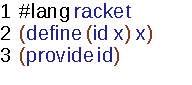
\includegraphics{untyped-rkt1.pdf}
\caption{untyped1.rkt: a simple Racket file}
\label{fig:ut1r}
\end{figure}

\begin{figure}
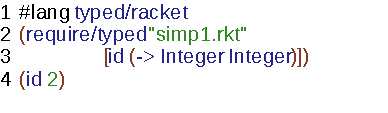
\includegraphics{typed-rkt1.pdf}
\caption{typed1.rkt: Typed Racket file using untyped1.rkt}
\label{fig:t1r}
\end{figure}

This construction, whereby every module is either entirely typed or entirely untyped
allows Typed Racket to take a unique approach to enforcement, built around
contracts CITEME applied at the points where modules interact. Types of values are
checked at boundaries, and methods are effectively wrapped as they cross between modules.

The key drawback to this approach is that a wrapper cannot establish \emph{actual
functionality} the same way that \emph{concrete} type systems can. Instead, wrapper
or guard based systems like the Typed Racket approach can only prove that a given untyped
function will \emph{act like} a typed function, up to cast errors.

As a demonstration of this, consider figure~\ref{fig:tr2}. TODO

\begin{figure}
Foo bar baz qux.
\caption{TODO Typed Racket example}
\label{fig:tr2}
\end{figure}

However, the use of promised typing provides a major advantage: untyped code does not 
need to be aware of types. In order to use a \emph{concrete} type system, even untyped
code must exist in at least an inheritance hierarchy that can be reasoned about by the 
runtime type checking system. As a result, promised typing can be used in languages that
do not have class hierarchies. 

While promised type systems can successfully type more code, they are limited in that
they cannot absolutely establish type correctness across casts, unlike concrete type
systems. As a result, errors occur when untyped code is used, rather than at the boundary
crossing.

\subsection{Reticulated Python}

Reticulated Python is an extension of Python adding sound gradual types by Michael 
Vitousek et al (CITEME), providing Python programmers with the ability to add types
to their programs. Unlike the other languages we have examined here, though, Reticulated
Python supports multiple different semantics for these types, providing different guarantees
and imposing different restrictions.

Three different gradual typing semantics are currently avaliable in Reticulated Python:
transient, monotonic, and guarded. All three systems are promised typing approaches,
checking to ensure that untyped code behaves as if it were typed from the perspective
of a typed observer. However, the mechanism for achieving this differs in each case.

\subsubsection{Guarded}

The guarded semantics for Reticulated Python is broadly similar to the semantics of
Typed Racket, as it uses wrappers to ensure that untyped code behaves as expected. 
However, it differs in one key area: where Typed Racket expects typed and untyped 
code to be in different compilation modules, the guarded semantics allows types
to be added anywhere in the program.

\begin{figure}
\begin{verbatim}
class A1:
  def a(a : Any) : Any:
    return a + 2
class A2:
  def a(a : Int) : Int:
    return a + 2

def test(a:A2):Int
  return a.a(2) + 1

test(A1())
\end{verbatim}
\label{fig:guard1}
\end{figure}

In figure~\ref{fig:guard1}, we see a correct program which runs successfully. Class A1
is dynamically typed, and class A2 is fully statically typed, while the test method
expects a statically typed instance of A2. We are then able to pass a dynamically typed
instance of class A1 into this test method as the guarded semantics will insert a wrapper
around A1 that makes sure it acts like an A2.

To see this more clearly, we can modify the above example into figure~\ref{fig:guard2}. Here,
A1 does not act like an A2 - when passed an argument, it will try and concatenate the string
``foo'' onto the end, and will return a string (if it can). As a result, we know that this will
produce an error, but the question is: where?

\begin{figure}
\begin{verbatim}
class A1:
  def a(a : Any) : Any:
    return a + "foo"
class A2:
  def a(a : Int) : Int:
    return a + 2

def test(a:A2):Int
  return a.a(2) + 1

test(A1())
\end{verbatim}
\label{fig:guard2}
\end{figure}

In this case, the error appears after the function A1.a returns, but before the value is passed
back to the caller. A wrapper is added around A1 that checks that the return value is an instance
of type int, and when it is not, an error is produced.

The guarded semantics is one of the most intuitive of the systems we have covered - errors are 
produced exactly when the value produced breaks the type guarantee. However, it suffers from the
same issues as were identified in TAKIAWA ET AL 2015 CITEME for Typed Racket, with considerable
``wrapper bloat'', caused when a value passes between typed and untyped code a large number of times.

\begin{figure}
\begin{verbatim}
class A1:
  def a(a : Any) : Any:
    return a + "foo"
class A2:
  def a(a : Int) : Int:
    return a + 2

def a1(a:A1):A1
  return a

def a2(a:A2):A2
  return a

a = A1()
for i=1,1000:
  a = a1(a2(a))
\end{verbatim}
\label{fig:guard3}
\end{figure}

This problem is illustrated in figure~\ref{fig:guard3}. The functions a1 and a2 act as casts to A1 and A2,
respectively, and we apply each to the same value 1000 times, alternating between a1 and a2. The problem 
here arises from the naive interpretation of wrapping, where each time we go from A1 to A2 we acquire a new
weapper. At the end of this program, a call to a would go through 1000 different objects!

While approaches to help simplify this particular problem exist, little progress has been made in eliminating
it entirely, at least to acceptible levels. As a concequence, two other systems have been added in Reticulated
Python that take a different perspective on the issue of how to ensure soundness, but at lower cost in memory
and levels of indirection.

\subsubsection{Transient}

In both the Strongscript and Typed Racket approaches, if you wrote a method (denoted $\m$ here)
under type $\int \rightarrow \int$, you could be assured that you would only ever be called
with an argument that was actually an int. To achieve this guarantee, the systems alternately
performed inline runtime casts based on runtime type information and inserted wrappers to
check that the types were respected \emph{before} an actual function call was made. Likewise,
a function that was declared to return an int would always return an int, ensured either by
wrapping or by adding casts inside of it.

Transient takes the opposite perspective. Instead of the caller being responsible for
checking the types on the arguments and the callee ensuring the return type is correct,
the transient semantics for Reticulated Python has the callee enforce the types on the
arguments and the caller enforce the type of the return value.

\subsubsection{Monotonic}
A key downfall of the approaches we discussed previously is that they
cause performance impacts in fully-typed code, especially at heap access
sites.The monotonic semantics for Reticulated Python aims to recover this,
in exchange for a new dynamically-enforced guarantee.

To see why the impact exists, consider the following code

\begin{verbatim}
function evil(x : *) : * {
	x := "foo bar"
}

Ref<Int> a = Ref(3)
evil(a)
Int y = !x + 2
\end{verbatim}

If we stripped all checks from this code, we would end up with a stuck
state, since we would be adding a string to an integer, despite statically
typing the value of $\a$ as an integer, as we were able to assign to the
underlying reference from an untyped context.

The approaches discussed for Typed Racket and the transient semantics
handle this case differently, but both require that the typed code perform
a typecheck at the dereference of $\x$. Problematically, these checks
have to be performed even in a fully typed program, because it is impossible
to know which pointers have been exposed to dynamic code.

The key feature of the monotonic semantics is that it imposes these checks 
on the dynamic code - any dynamic reference has to respect the types imposed
by a typed reference. In the above example, the monotonic semantics would
produce an error when we tried to assign a string into $\x$ - despite the 
static typing working out, because the reference has a type which is incompatible
with our new type, monotonic will reject it at that point.
%%%%%%%%%%%%%%%%%%%%%%%%%%%%%%%%%%%%%%%%%%%%%%%%%%%%%%%%%%%%%%%%%%%%%%%%%%%
\section{A Common Core for Gradually Typed Objects}

These type systems represent a cross section of approaches taken in defining
gradual typing. However, they are all designed for and implemented on different
underlying languages, creating difficulties in comparing them, and motivating
our use of generalizations and text to describe them.

This section introduces the small object calculus we use to illustrate the
differences between the four gradual type systems.  The calculus was
carefully designed to act as a common core on top of which gradual type
systems can grafted with relative ease. As usual in such exercises, we aimed
for minimality, language features not directly required for our development
were omitted. The result is an imperative class-based system that does not
support inheritance. The calculus adopts a very simple structural type
system with concrete types and a single unconstrained type.

The common core allows writing traditional object-oriented examples such as
a typed \xt{Point} class.\footnote{For our examples we use integers and
  common arithmetic operations even if they are not in core calculus.}

%%% FIXME: formatting
\begin{verbatim}
class Point {
  x : Int
  y : Int
  addx( v : Int ) : Int {
       this.x!( this.x() + v )
  }
  addy( v : Int ) : Int {
       this.y!( this.y() + v )
  }
}
\end{verbatim}

The type system ensures that, if \xt{pt} is declared to be of type
\xt{Point}, an operation such as \xt{pt.addx(42)} will not get stuck.  As
this small language requires all variables to be initialized, there checking
for \xt{null} is not needed as it likely would in a full fledged language.

The language also supports a single unconstrained type, denote \any (pronounced
dyn), thus one could write the following method

%%% FIXME: formatting
\begin{verbatim}
  mkPt( u : * ) : Point {
      new Point( u.x() 
                 (<Point> u).y() )
  }
\end{verbatim}

This method will accept an instance of any class and will return a new
\xt{Point}. At run-time, the code will get stuck if the dynamic cast
\xt{\Cast{\xt{Point}}{\xt{u}}} fails. If \x is a declared of type \any, an
expression such as \xt{u.x()} will fail if the object bound to \xt{u} does
not have a getter \xt{x()}.


For brevity we use annotate variables with nominal types, but in the
calculus this is merely shorthand for writing the set of methods suported 
by the class. Assignment to fields is performed by automatically generated
getter and setter methods.

The syntax of the common core appears in figure~\ref{syn}.  \x ranges
over variables, \f ranges over field names, \m can be either a plain method
name \d, a field getter \f, or a field setter \fb, \C and \D range over
class names. We use the overbar notation to denote a possibly empty
sequence. In the common core, a class is defined as by a set of fields,
\b\f, with distinct names and a set of method definitions, \b\m. An instance
of class is constructed by the expression \New\C{\b\e} where each argument
is used to initialize the corresponding field. Fields are encapsulated and
can only be accessed and updated in the corresponding getter and setter from
the \this variable.  Expressions include variable access, field access and
update, method invocation, object creation, and type casts.



%%%%%%%%%%%%%%%%%%%%%%%% SYNTAX %%%%%%%%%%%%%%%%%%%%%%%%%%%%%%%%%%%%%%%%%%%%%%%%
\begin{figure}[!h]\center\begin{minipage}{4cm}\begin{tabular}{l@{~~~}l}
\e &::=  \x \\
%   \Alt{ \Get\e\f }
%   \Alt{ \Set\e\f\e }
   \Alt{ \Call\e\m{\b\e} }
   \Alt{ \New\C{\b\e} }
   \Alt{ \Cast\t\e }
\fd &::= 
    \Ftype\f\t   \\
\end{tabular}\end{minipage}\begin{minipage}{4cm}\begin{tabular}{l@{~~~}l}
\md &::=
    \Mdef\m\x\t\t\e \\
\c &::= \Class \C {\b{\fd}}{\b{\md} } \\
\mt &::= \Mtype\m{\b\t}\t\\
\t &::= ~ \any \\
   \Alt{ \Type{  \b{ \mt } } }
   \Alt\C \\
\end{tabular}\end{minipage}
\caption{Abstract Syntax for the Core Calculus}\label{syn}
\end{figure}
%%%%%%%%%%%%%%%%%%% END OF SYNTAX %%%%%%%%%%%%%%%%%%%%%%%%%%%%%%%%%%%%%%%%%%%%%%

Our types are structural and only account for the methods in an object's
interface. For type annotations, we use the name of classes, ranged over by
\C and \D, as shorthand for the set of methods defined in the respective
classes.


%%%%%%%%%%%%%%%%%%%%%% DYNAMIC SEMANTICS %%%%%%%%%%%%%%%%%%%%%%%%%%%%%%%%%%%%%%
\begin{figure}

\begin{minipage}{8cm}
\opdef{\Reduce{\ep 1}{\sp 1}{\ep 2}{\sp 2}}{\ep1 \sp1 evaluates to \ep2 \sp2 or \err in a step}\\[-1mm]
\begin{tabular}{@{}l@{}l@{~}l@{~}l}
\CondRule{E1}{ %% e -> e'
  \Reduce {\ep 1}{\sp 1}{\ep 2}{\sp 2}
}{
  \ReduceA {\Ctx{\ep1}}{\sp 1}{\Ctx{\ep2}}{\sp 2}
}
\CondRule{E2}{ %% new C -> a
   \alloc{\sp2}{\ap1}{\sp1}{\Obj{\b\a}\C}
}{ 
    \ReduceA{ \New\C{\b\a} }{\sp1}{\ap1}{\sp 2}
}
\CondRule{E3}{ %% a.m -> e
   \dispatch{\b\x}\e\s\a\m
}{
   \ReduceA{\Call\a\m{\b{\ap 1}}}\s{[\a/\this~\b{{\ap 1}/\x}]\e}\s
}

\CondRule{E3}{
   \notdispatch{\b\x}\e\s\a\m
}{
   \ReduceA{\Call\a\m{\b{\ap 1}}}\s{\err}{}
}
\CondRule{E3}{ 
     \readfield{\ap1}\s\a\f
}{
  \ReduceA{\Get\a\f}{\s}{\ap 1}{\s}
}
\CondRule{E4}{
     \setfield{\sp2}{\sp1}\a\f{\ap1}
}{
     \ReduceA{\Set\a\f{\ap 1}}{\sp 1}{\ap 1}{\sp 2}
}
\NoCondRule{E5}
{ 
   \ReduceA{ \Cast\any\a}\s \a\s
}
\CondRule{E6}{
  \typeof\s\a \Sub \tp 1
}{ 
    \ReduceA{\Cast{\tp 1}\a}\s\a\s
}
\CondRule{E7}{
  \typeof\s\a \NotSub \tp 1
}{ 
    \ReduceA{\Cast{\tp 1}\a}\s\err{}
}
\CondRule{E8}{
    \Reduce\e{\sp 1}\err{}
}{
    \ReduceA{\Ctx\e}{\sp1}\err{}
}
\end{tabular}\end{minipage}
%%%%%%%%%%%%%%%%%%% CONTEXTS %%%%%%%%%%%%%%%%%%%%%%%%%%%%%%%%%%%%%%%%%%%%
\\[3mm]
\begin{minipage}{4cm}\begin{tabular}{l@{~~}l@{~}l}
\s &::= ~~\none & \B ~~
  \Heap\s{\Bind\a{\Obj{\b\a}{\t}}} \\[2mm]
\xt{E} &::=    \Get\square\f &\B~
       \Set\square\f\e   ~\B~
       \Set\a\f\square   ~\B~  
       \Call\square\m\e  ~\B~
      \Call\a\m{\b\a\,\square\,\b\e} \\
 &\B~     \Cast\t\square  &\B~
      \New\C{\b \a\,\square\,\b\e}
\end{tabular}
\end{minipage}
\caption{Common Core Calculus Dynamic Semantics.}
\end{figure}

The dynamic semantics evaluates expression extended with object references,
denoted \a, and errors, denoted \err, together with a heap \s mapping
references to object values. Object values contain all fields, methods, a
type, and a class; they are denoted \Obj{\b\a}\C. The
class is used for locating methods and the type is used for type casts. The
need for keeping them separate will become clear later.

The semantics uses evaluation context \Ctx\e.

Selecting an object from the heap is written \Sel\s\a, while a heap is
extended with a new object by \Heap{\s}{\Bind{\a}{\Obj{\dots}\C}}.


For an object reference \a, such that \M{\Sel\s\a=\Obj{\dots}\C}, we have 
\classofis{\Sel\s\a}\C and \typeofis\s\a\t.

We use the notation \Mdef\m\x\t\t \inc\C to select a method in a class
definition and \Fdef\f\t\a\inc\Obj{\dots}\C to express the selection of a
field. Lastly a field of an object can be update with the notation
\Update{\Obj{\dots}\C}\f\a.

\subsection{Core Type System}

Using this dynamic semantics, we can then define a simple, sound, type system
that ensures that well-typed programs will not get stuck, seen in figure~\ref{fig:basetyp}.

Our basic type system is typical of calculi that support objects, notably including 
subtyping. Subtyping in our system is defined in figure~\ref{fig:sub}, which
defines a simple structual subtyping system with names (to provide for recursive types)
as well as the Amber rule to support recursive types. Notably, however, because there
are no valid operations on $\any$ other than casting, this type system cannot be called
a \emph{gradual} type system.

%TODO: Explain what's up with sigma

Soundness for this base system is typical, though we define it through combining 
the progress and preservation lemmas to enable a special case, whereby only casts
can possibly fail.

\begin{thm}
If $\EnvType\Es\e\t$, then one of the following holds:
\begin{itemize}
\item $\e \rightarrow \e'$ and $\EnvType\Es{\e'}\t$
\item $\e \rightarrow \xt{v}$ and $\EnvType\Es{\xt{v}}\t$
\item $\e$ is $\Cast{\t}{\e'}$ and $\e \rightarrow \err$
\end{itemize}
\end{thm}

This core, sound, completely typed calculus provides the requisite guarantee,
that well typed programs will not get stuck, but does very little for gradual
typing, as it requires that a programmer insert a large number of casts in order
to interact with code of type $\any$.
\begin{figure}
\opdef{\EnvType{\Es}\e\t}{\e has type \t in environment \E against heap \s}
\begin{mathpar}
\IRule{W1}{
    \HasType{\E}\x\t
 }{
   \EnvType{\Es}\x\t
}

\IRule{W2}{
   \EnvType{\Es}\e{\tp 1} \\ \tp 1 \Sub \t
 }{
   \EnvType{\Es}\e\t 
}   

\IRule{W4}{
   \EnvType{\Es}\e{\C} \\ \Mtype\m{\b{\tp2}}\t\inc \C  \\  \b{\EnvType{\Es}{\ep1}{\tp 2}}
}{
    \EnvType{\Es}{\Call\e\m{\b{\ep1}}}\t
}    

\IRule{W5}{
  \b{\EnvType{\Es}\e\t} \\ 
  \Class \C {\b{\Ftype\f\t}} {\b{\md}}
}{
  \EnvType{\Es}{\New\C{\b\e}}\C
}

\IRule{W6}{
  \EnvType{\Es}\e{\tp1}
}{
   \EnvType{\Es}{\Cast\t\e}\t
}

\IRule{W7}{
  \EnvType{\Es}{\ep1}{\tp1} \\
  \f : \t \in \tp1 \\
}{
  \EnvType{\Es}{\Get\e\f}{\t}
}

\IRule{W8}{
  \EnvType{\Es}{\ep1}{\tp1} \\
  \f : \t \in \tp1 \\
  \EnvType{\Es}{\ep2}{\t}
}{
  \EnvType{\Es}{\Set{\ep1}\f{\ep2}}\t
}

\IRule{W9}{
  \s(\ap1) = \Obj{\b{\f=\ap2}}{\C} \\ \b{\f:{\tp2} \in \C} \\ \b{\EnvType{\Es}{\ap2}{\tp2}} \\ 
}{
  \EnvType{\Es}{\ap1}{\tp1}
}
\end{mathpar}
\caption{Typing rules for the base langauge}
\label{fig:basetyp}
\end{figure}



\section{Gradual Typing}
In order to extend the core calculus to enable programmers to write gradually
typed code without having to insert a great number of casts manually, we
use gradual type systems to add casts where required, presenting a unified gradual
semantics to the programmer while relying on the core system for soundness.

Our characterization of gradual typing is \emph{gradual typing by translation},
using an approach similar to that of (MEIJER ET AL CITEME), adding gradual
types to the underlying fully typed language. In this vein,
we define our gradual typing extensions as \emph{cast insertion} phases.

This approach lets us simply present the working mechanism of the type
systems. For each of the systems in question, we present the cast insertion
mechanism required to convert a gradually typed program into a fully typed
program with casts respecting the guarantee of the gradual typing system in
question, and demonstrating the workings of each system.

However, the systems share a considerable amount of their basic semantics.
To prevent needless duplication, we use a \emph{common core} of translation
rules, which we then modify or extend to support the gradual typing system in
question.

\subsection{Cast Insertion}

The user-facing component of a gradual typing system is its type checker,
or the surface type system, which is then complemented by a type-driven
cast insertion mechanism ``behind the scenes''. In our approach, these two
steps are combined into a cast insertion system.

Cast insertion is fundamentally \emph{type driven}. In our type system, it is
required to have a cast whenever a type needs to be altered, and therefore in
inserting casts we need to know every site where one type is required to be another.
Our system handles this through an \emph{bidirectional cast insertion} system,
introduced by (PIERCE AND TURNER CITEME).

Our choice comes from an observation about the nature of traditional bottom-up type
systems. The fundamental building block is judgements of the form $\E \vdash \e : \t$, 
which means that $\e$ inherently has type $\t$. For example, a type mismatch
would look like trying to conclude a judgement $\E \vdash \e : \any$ when only
$\E \vdash \e : \xt{int}$ holds.

Other systems have solved this problem through the introduction of nondeterministic
rules such as subsumption, but nondeterminism in cast insertion creates problems
where a single program can be typed in multiple different ways (EXAMPLE).

To solve this problem, we use the aforementioned bidirectional cast insertion
mechanism. In a bidirectional system, we have two judgements:

\begin{itemize}
\item The \emph{analytic} judgement $\E \vdash \e \Rightarrow \t$, which says that
$\e$ inherently has type $\t$ against environment $\E$, equivalently to the
traditional bottom-up type system.
\item The \emph{synthetic} judgement $\E \vdash \e \Leftarrow \t$, which implies that
$\e$ can potentially have type $\t$ against environment $\E$.
\end{itemize}

For example, consider the function call $\Call{\ep1}{\m}{\ep2}$. A bidirectional
type system will begin with seeing what type $\ep1$ has, with the judgment $\E \vdash \ep1 \Rightarrow \t$.
From this, the bidirectional type system will check what type the method $\m$ has in $\t$,
 here denoted $\Mtype\m{\tp1}{\tp2} \in \t$, then ensure that the arguments make sense with that type.

In a bottom-up type system, we would write $\E \vdash \ep2 : \tp1$, but, as commonly noted with subsumption,
this can require the introduction of a nonalgorithmic rule to conclude this final judgment. Instead, in a 
bidirectional type system, we can simply ensure that the type of $\ep2$ is consistent with $\tp1$ through the
judgment $\E \vdash \ep2 \Leftarrow \tp2$.

Finally, we will be able to conclude that $\E \vdash \Call{\ep1}{\m}{\ep2} \Rightarrow \tp2$. This is a
synthetic judgement as $\tp2$ is the type that the expression can be known to have in the absence of any
external information.

To support cast insertion, we extend these basic type checking judgements with an output term, of the form 
$\GenCast{\E}{\ep1}{\ep2}{\t}$ for the synthetic case and $\AnaCast{\E}{\ep1}{\ep2}{\t}$ for the analytic,
case, where the former translates $\ep1$ to $\ep2$ producting type $\t$, and the latter translates the same
ensuring type $\t$.

An important note in the construction of our bidirectional type system is that our handling of the key case,
function application, is less specific than it could be, as we ignore the analytic case. Other works in this 
area, including (DUNFIELD \& KRISHNASWAMI CITEME) use a third bidirectional judgment to handle function 
application, largely to handle the analytic case. If we are trying to typecheck a function call against some 
known type, then we can infer a type for the receiver by using synthetic type checking on the arguments. 
However, in our context, detailed handling of this case is not required, as our type inference does not 
need to be as precise as it does for (DUNFIELD ET AL's) type inference.

\subsection{Class Translation}

A key component of many gradual type systems is enabling checks for every field access or modification,
ensuring type invariants about the heap. To enable these checks, we cannot expose ``raw'' field access
and modification in our calculus, as otherwise these checks could be easily bypassed.

As a result, we expose no typing judgment for field manipulation, and instead auto-generate getter and 
setter methods in a phase we call \emph{class translation}, occuring at the same time as cast insertion.

Another issue solved by class translation is that raised by calling a method on a dynamic receiver type.
Consider the invocation $\Call{\e}{\m}{\e'}$ where $\EnvType{\Es}{\e}{\any}$ and $\EnvType{\Es}{\e'}{\any}$. 
Now, suppose that we have a method on $\e$ $\m(\x:\C)$. Using casting, we can figure out that the method exists,
and that the arity is correct, but there is no static way to know the argument types of $\m$ statically to 
insert checks.

Class translation solves this problem by creating a ``guard'' method $\m_\xt{u}$ that will have the same
arity and a related name, but only has arguments of type $\any$. We then translate every call to a method
$\m$ on an untyped receiver to a call to a call to $\m_\xt{u}$, which then does the approperiate type check
before calling the typed method.

%%%%%%%%%%%%%%%%%%%%%%%% SUBTYPING %%%%%%%%%%%%%%%%%%%%%%%%%%%%%%%%%%%%%%%%
\newcommand{\ESub}[3]{#1 \vdash #2 \leq #3}

\begin{figure}
\opdef{$\tp1 \Sub \tp2$}{\tp 1 is a subtype of \tp 2}
\opdef{$\ESub{\Xi}{\tp1}{\tp2}$}{\tp 1 is a subtype of \tp 2 against environment $\Xi$}
\begin{mathpar}
\IRule{L1}{\ESub\emptyset{\tp1}{\tp2}}{\tp1 \Sub \tp2}

\IRule{S1}{}{\ESub\Xi\t\t}

\IRule{S2}{}{\ESub\Xi\t{\Type{}}}

\IRule{S3}{\vdash \C : \tp2 \\ \ESub\Xi{\tp2}{\tp1}}{\ESub\Xi\C{\tp1}}

\IRule{S4}{\vdash \C : \tp2 \\ \ESub\Xi{\tp1}{\tp2}}{\ESub\Xi{\tp1}\C}

\IRule{S5}{
  \tp1 \leq \tp2 \in \Xi
}{
 \ESub{\Xi}{\tp1}{\tp2}  
}

\IRule{S6}{
    \Xi' = \Xi,~{\t \leq \Type{\Mtype\m{\b{\tp1}}{\tp2} ~ \b{\mt} \,}} \\
    \ESub{\Xi'}\t{\Type{\b{ \mt } }}\\
     \Mtype\m{\b{\tp3}}{\tp4} \inc \t \\
    \b{\ESub{\Xi'}{\tp3}{\tp1}} \\
    \ESub{\Xi'}{\tp2}{\tp4} \\    
}{
   \ESub\Xi\t{\Type{\Mtype\m{\b{\tp1}}{\tp2} ~ \b{\mt} \,} } 
}
\end{mathpar}
\caption{Subtyping}
\label{fig:sub}
\end{figure}


%%%%%%%%%%%%%%%%%%%%%%%%% WELLFORMDNESS %%%%%%%%%%%%%%%%%%%%%%%%%%%%%%%%%%


\begin{figure}
\opdef{$\GenCast\E{\ep1}{\ep 2}\t$}{\ep1 translates to \ep2 in environment \E with type $\t$}
\begin{mathpar}
\IRule{A1}{\HasType{\E}\x\t}{\GenCast\E\x\x\t}

\IRule{A4}{
	\GenCast{\E}{\e_1}{\e_2}{\t_1} \\
	\Mtype\m{\b{\tp 2}}{\tp 3} \inc \t_1\\
	\b{\AnaCast{\E}{\e_3}{\e_4}{\tp 2}} \\
}{
	\GenCast{\E}{\Call{\e_1}\m{\b{\e_2}}}{\Call{\e_3}{\m}{\b{\e_4}}}{\tp 3}
}

\IRule{A5}{
	\GenCast{\E}{\e_1}{\e_3}{\any} \\
	\b{\AnaCast{\E}{\e_2}{\e_4}{\any}} \\
}{
	\GenCast{\E}{\Call{\e_1}\m{\b{\e_2}}}{\Call{\Cast{\Type{\Mtype{\m_\xt{u}}{\b{\any}}\any}}{\e_3}}{\m_\xt{u}}{\b{\e_4}}}{\any}
}

\IRule{A6}{
  \b{\AnaCast\E{\e_1}{\e_2}\t} \\ 
  \Class \C {\b{\Ftype\f\t}} {\b{\md}}
  }{\GenCast{\E}{\New\C{\b{\e_1}}}{\New\C{\b{\e_2}}}{\C}}
\end{mathpar}
\caption{Synthetic cast insertion}
\end{figure}

%%%%%%%%%%%%%%%%%%%%%%%%% CLASS TRANSLATION %%%%%%%%%%%%%%%%%%%%%%%%%%%%%
\begin{figure}
\opdef{$\AnaCast\E{\ep1}{\ep 2}\t$}{\ep1 translates to \ep2 in environment \E with type $\t$}
\begin{mathpar}
\IRule{AASC2}{
  \GenCast{\E}{\ep1}{\ep2}{\tp2} \\
  \tp2 <: \tp1\\
}{
  \AnaCast{\E}{\ep1}{\ep2}{\tp1}
}

\IRule{AASC3}{
  \GenCast{\E}{\ep1}{\ep2}{\any} \\
}{
  \AnaCast{\E}{\ep1}{\Cast\any{\ep2}}{\any}
}
\end{mathpar}
\caption{Analytic Cast Insertion}
\end{figure}

\begin{figure}
\opdef{\TransExp\E{\ep1}{\ep 2}\t}{\ep1 translates to \ep2 in environment \E with type $\t$}
\begin{mathpar}
\IRule{CT1}{
 \b{ \mdp1} \equiv \b{\fcast{\md}} ~~ \b{\setter\fd} ~~ \b{\getter\fd}\\  \b{\mdp2} \equiv \b{\mdp1} ~~ \b{\proxy{\mdp1}}
}{ 
  \TransClass { \Class \C {\b{\fd}} {\b{\md}} }{  \Class \C {\b{\fd}} {\b{\mdp2}} }
}

\IRule{}{
  \AnaCast{\b{\x:\tp1}}{\ep1}{\ep2}{\tp2}
}{
  \fcast{\Mdef\m\x{\tp1}{\tp2}{\ep1}} \equiv \Mdef\m\x{\tp1}{\tp2}{\ep2}
}

\IRule{}{
}{
  \getter{\f:\t} \equiv \m() : \t ~ \{ \this.\f \}
}

\IRule{}{
}{
  \setter{\f:\t} \equiv \m(\x:\t) : \t ~ \{ \this.\f=\x \}
}

\IRule{}{
}{
  \proxy{\Mdef\m\x{\tp1}{\tp2}{\ep1}} \equiv \Mdef{\m^*}\x{\any}{\any}{\Cast{\any}{\Call\this\m{\b{\Cast{\tp1}\x}}}}
}
\end{mathpar}
\caption{Class Translation}
\end{figure}
%%%%%%%%%%%%%%%%%%%%%%%%%%%%%%%%%%%%%%%%%%%%%%%%%%%%%%%%%%%%%%%%%%%%%%%%%


\subsection{Type soundness:}
Theorem 1: Type translation. If $\EnvType{\Es}\e\t$ and $\TransExp\E\e{\e'}\t$ then $\EnvType{\E ~ \cdot}{\e'}\t$.

Theorem 2: Progress. If $\EnvType{\Es}{\e}{\t}$ then $\s,\e \rightarrow \s',\e'$ for $\e'$ expression or $\e' ~ \err$.

Theorem 3: Preservation. If $\s,\e \rightarrow \s',\e'$ and $\EnvType{\Es}{\e}{\t}$ then $\EnvType{\E~\s'}{\e'}{\t}$.

For a list of classes $\bar{\c}$ such that $\b{\c ~~ WF}$ and an expression $e$ such that $\EnvType\cdot\e\t$ and $\b{\TransClass\c{\c'}}$, we have $\cdot~e \rightarrow^* \sigma~r$ (against $\b{\c'}$) where $r$ is either a value or $\err$.


\begin{figure}
\begin{mathpar}
\IRule{TRNew1}{
  \b{\AnaCast\E{\e_1}{\e_2}\t} \\ 
  \Class \C {\b{\Ftype\f\t}} {\b{\md}} \\
  \typed{\C}
  }{\GenCast{\E}{\New\C{\b{\e_1}}}{\New\C{\b{\e_2}}}{\C}}

\IRule{TRNew2}{
  \b{\AnaCast\E{\e_1}{\e_2}\any} \\ 
  \Class \C {\b{\Ftype\f\any}} {\b{\md}} \\
  \untyped{\C}
  }{\GenCast{\E}{\New\C{\b{\ep1}}}{\Cast{\any}{\New\C{\b{\ep2}}}}{\any}}

\IRule{AASC1}{
  \GenCast{\E}{\ep1}{\ep2}{\t} \\
  \t \neq \any \\
  \C = \utw{\t}
}{
  \AnaCast{\E}{\ep1}{\Cast{\any}{\New\C{\ep2}}}{\any}
}

\IRule{AASC2}{
  \GenCast{\E}{\ep1}{\ep2}{\any} \\
  \t \neq \any \\
  \C = \tw{\t}
}{
  \AnaCast{\E}{\ep1}{{\New\C{\ep2}}}{\t}
}

\IRule{MTWrap}{
}{
  \tw{\Mtype\m{\b{\tp1}}\t} = \Mdef\m\x{\tp1}{\t}{\Cast{\t}{(\Cast{\Type{\Mtype{\m_\xt{u}}{\b\any}{\any}}}{\this.\xt{s}}).\m_\xt{u}(\b{\Cast{\any}{\x}})}}
}

\IRule{MUTWrap}{
}{
  \utw{\Mtype{\m}{\b{\tp1}}\t} = \Mdef{\m^\xt{*}}\x{\any}{\any}{\Cast{\any}{\this.\xt{s}.\m(\b{\Cast{\tp1}{\x}})}}
}

\IRule{TWrap}{
  \Class\C{\xt{s} : \any}{\b{\tw{\mt}}}
}{
  \tw{\Type{\b{\mt}}} = \C
}

\IRule{TUWrap}{
  \Class\C{\xt{s} : \Type{\b{\mt}}}{\b{\utw{\mt}}}
}{
  \utw{\Type{\b{\mt}}} = \C
}
\end{mathpar}
\caption{Translation for Typed Racket}
\end{figure}

Typed Racket uses a much stricter definition of where $\any$ types can go, where every class is either fully typed or fully untyped. To describe this, we alter definition 1 and 2 to


\begin{definition} A Typed Racket class table is well-formed if for every class \C  in
the class table, every method is of the form \Mdef\d\x{\tp1}{\tp2}\e where
\EnvType{\this:\C,\b{\x:\tp1}}\e{\tp2} holds in \C, and all types in \C are either $\any$ or all not $\any$
\end{definition}

Typed Racket uses wrappers to ensure that typed code type guarantees are not violated, and that untyped code follows the types that it is casted to. We generate these wrappers using the following mechanism.

\begin{definition}
Every place a type \Type{\mt} where $\mt=\Mtype\m{\b{\tp1}}{\tp2}$ flows from typed into untyped code, generate a wrapper $\Class{\C'}{~\xt{orig}:\t,\b{\md}}$ where $\md = \Mdef\m\x{\any}{\any}{\Cast{\any}{\xt{this}.\xt{orig}.\m(\b{\Cast{\tp1}x})}}$.
\end{definition}

To model Typed Racket, we then need to enforce the property that objects are wrapped at typed/untyped boundaries, and ensuring that untyped code cannot use typed code internally through casts. We do this by altering the completion process, giving us a new definition. We use the wrappers we generated using definition 4 to enforce the type guarantees
\newpage
\begin{definition} A Typed Racket class table is completed if for every 
 \Class \C {\b{\fd}} {\b{\md}} in the class table: 
 \begin{itemize}
 \item for every type \Type{\b{\md}}, add a class \xt{D} such that 
 \begin{itemize}
 \item for every method $\Mtype\m{\tp1}{\tp2} \in \b{\md}$, generate a function in \xt{D} $\Mdef\m{x}{\any}{\any}{\Cast{\any}{\New{\xt{D}}{\xt{this}.\xt{orig}.\m(\New\C{\b{\Cast{\tp1}x}})}}}$
 \end{itemize}
 \item for every field \Ftype\f\t\inc\C, we add to \C:
 \begin{itemize}
 \item A setter \SMdef\f\x\t\t{\Set\this\f\x} 
 \item A getter \GMdef\f\t{\Get\this\f}; 
 \end{itemize}
 \item For every method definition \Mdef\d\x\t{\tp1}\e\inc\C:
 \begin{itemize}
 \item A dynamic method \Mdef{\Dyn\d}\x\any\any{\Cast\any{\Call\this\d{\b{\Cast\t\x }} }} is added to \C 
 \item We replace the body \e of \m is replaced by \ep1 where \TransClass\e{\ep1}.
 \end{itemize}
 \end{itemize}
\end{definition}

One of the issues inherent to the Strongscript approach (and is apparent in
the common core as well) is that a strict interpretation of the static type
system causes the programmer to have to write a very large number of
``obvious'' casts, breaking untyped code and seemingly-sensible typed
code. We can solve this by having the compilation process insert the types
for the programmer, which we describe using a cast insertion system.

Our cast insertion approach is based on a bidirectional type
system~\cite{}, where each expression either \emph{synthesizes}, or
inherently makes, a type, or is \emph{analyzed} against a type where the
type system checks to make sure that the expression still ``works'' under
the given type. This approach has been used for a number of other tasks,
including inferring types to select sub-languages~\cite{}, infer
types for higher rank languages~\cite{}. In our case, they allow us
to simply specify in an extensible manner where to insert casts.

Synthetic cast insertion is closer to a traditional type system, as it produces types from terms in a similar manner. However, instead of having non algorithmic cases where types are known (for example, in the arguments to a typed function), the synthetic cast insertion judgment defers to the analytic cast insertion mechanism with the known type. Importantly for us, the basic semantics of the static type system does not change between any of the type systems under consideration, and as a result the synthetic cases are not changed by any of the systems.

Analytic cast insertion ensures that an expression is of a given type. We use analytic cast insertion when a type is known for an expression and we want to force that expression to be of the correct type, which we do by inserting the appropriate cast. The actual details of analytic cast insertion vary depending on the system under consideration (most notably, the monotonic semantics has a notion of consistency that differs from the other two systems).

\begin{figure}

$\t = \ldots \B {\WType{\Mtype\m\t\t}}$

\begin{mathpar}
\IRule{STS1}{
}{
	\tp1 \Sub \Weak\tp1
}

\IRule{STS2}{
	\tp1 \Sub \tp2
}{
	\Weak\tp1 \Sub \Weak\tp2
}

\IRule{A5}{
	\GenCast{\E}{\e_1}{\e_3}{\Weak\tp1} \\
	\Mtype{\m}{\tp2}{\tp3} \in \tp1 \\
	\b{\AnaCast{\E}{\e_2}{\e_4}{\Weak\tp2}} \\
}{
	\GenCast{\E}{\Call{\e_1}\m{\b{\e_2}}}{\Call{\Cast{\Type{\Mtype{\m_\xt{u}}{\b{\any}}\any}}{\e_3}}{\m_\xt{u}}{\b{\e_4}}}{\Weak\tp3}
}

\IRule{AASC1}{
  \GenCast{\E}{\ep1}{\ep2}{\Weak\tp2}
}{
  \AnaCast{\E}{\ep1}{\Cast{\tp1}{\ep2}}{\tp1}
}

\IRule{AASC2}{
  \GenCast{\E}{\ep1}{\ep2}{\tp2}
}{
  \AnaCast{\E}{\ep1}{\Cast{\any}{\ep2}}{\Weak\tp1}
}
\end{mathpar}
\caption{Strongscript}
\end{figure}

\begin{figure}
\begin{mathpar}
\IRule{A5}{
	\GenCast{\E}{\e_1}{\e_3}{\tp1} \\
	\Mtype{\m}{\b{\tp2}}{\tp3} \in \tp1 \\
	\b{\AnaCast{\E}{\e_2}{\e_4}{\tp2}} \\
}{
	\GenCast{\E}{\Call{\e_1}\m{\b{\e_2}}}{\Cast{\tp3}{(\Call{\e_3}{\m_u}{\b{\Cast{\any}{\e_4}}})}}{\tp3}
}
\end{mathpar}
\caption{Transient}
\end{figure}

\clearpage
\newpage

\section{Monotonic}

%%%%%%%%%%%%%%%% Monotonic Statics

\begin{figure}[h]
\begin{mathpar}
\IRule{CS1}{ }{\stcons{\t}{\t}}

\IRule{CS2}{ }{\stcons{\any}{\t}}

\IRule{CS3}{ }{\stcons{\t}{\any}}

\IRule{CS4}{ \tp 1 \Sub \tp 2 }{\stcons{\tp 1}{\tp 2}}

\IRule{CS5}{
    \Mtype\m{\b{\tp1}}{\tp2} \in \t\\
	\b{\stcons{\tp3}{\tp1}} \\
    \stcons{\tp2}{\tp4} \\
    \stcons{\t}{\Type{\b{\md}}}
}{\stcons{\t}{\Type{\Mtype\m{\b{\tp3}}{\tp4} ~ \b{\md}}}}
\end{mathpar}
\caption{Consistent Subtyping}
\end{figure}

The key static difference between the monotonic semantics and the other systems we have considered is the consistent subtyping relationship. Traditional subtyping can be thought of as if a value satisfies one type, then it will satisfy any supertype of that type. Consistent subtyping encapsulates both this notion and the new idea of consistency. Consistency for objects means that two types have static type information that does not conflict - e.g. $\Type{\Ftype\f\any}$ could very well be able to replace $\Type{\Ftype\f\C}$, though we are unable to tell statically. Consistency allows us to interchange these types, inserting a cast where required.

Subtype consistency combines the two properties. Subtyping lets us add and remove fields from a type, and consistency allows us to make the type we are going to more or less dynamic. Going by the above intuition, a value of type $\any$ could work with any other type and vice versa, and clearly two identical types are compatible. The most complex case is when we have two class types, both with the same method $\m$, which we resolve by ensuring that $\m$ has parameters and return types that are consistent and continuing on through the rest of the class.

Adding this to our static type system is simple. We just introduce the rule that allows types to be converted via $\stcons{}{}$. The details of how to make the dynamics work with this static addition will be covered later.

\begin{figure}[h]
\opdef{$\meet{\tp1}{\tp2} \equiv \tp3$}{The most specific type common to $\tp1$ and $\tp2$ is $\tp3$}
\begin{mathpar}
\IRule{M1}{ }{\meet{\t}{\any} \equiv \t}

\IRule{M2}{ }{\meet{\any}{\t} \equiv \t}

\IRule{M3}{ }{\meet{\t}{\t} \equiv \t}

\IRule{M4}{
	\b{\meet{\tp3}{\tp1}  \equiv \tp5} \\
    \meet{\tp2}{\tp4} \equiv \tp6\\
    \meet{\Type{\b{\md_1}}}{\Type{\b{\md_2}}} \equiv \Type{\b{\md_3}} 
}{\meet{\Type{\Mtype\m{\b{\tp1}}{\tp2}~ \b{\md_1}}}{\Type{\Mtype\m{\b{\tp3}}{\tp4} ~ \b{\md_2}}} \equiv \Type{\Mtype\m{\b{\tp5}}{\tp6} ~ \b{\md_3}}}
\end{mathpar}
\caption{Meet for the monotonic system}
\end{figure}

This idea leads us into the core of the monotonic idea. Under this system, if we have a field of some given type $\t$, we do not know if the value of that field is truly of the expected type (since the class could have been cast to one where that field is $\any$ and the field updated), and therefore have to check the value of $\f$ at every point it is used. The solution used by the monotonic approach is to ensure that if a type is given to a field, then that type is never violated.

Consistency allows us to convert between, for example, $\Type{\Ftype\f\any, \Ftype{\xt{g}}\C}$ and $\Type{\Ftype\f\C, \Ftype{\xt{g}}\any}$, as neither has static typing information that would rule out a value that satisfied the other type. However, if we have a value that satisfied both, we would end up with a type that had neither type exactly - we would have $\Type{\Ftype\f\C, \Ftype{\xt{g}}\C}$. This is the key to the monotonic system - we never throw away any type information away. If, at any point in the program, we have an object with some specialized (e.g. not all $\any$) type, then those type assumptions will never be violated. As a result, we can ensure that no get operation will need to be checked.

\begin{figure}
\begin{mathpar}
\IRule{AA2}{\GenCast{\E}{\ep1}{\ep2}{\tp 2} \\ \tp2 \not\Sub \tp1 \\ \stcons{\tp2}{\tp1}}{\AnaCast\E{\ep1}{{\Cast{\tp1}{\ep2}}}{\tp1}}
\end{mathpar}
\caption{Analytic cast insertion}
\end{figure}


\begin{figure}

Index every type $\t$ in the source of the program with an index $i$ (denoted $\t^i$). Then, for every class $\C$ and every $i$ where $\stcons\c{\t^i}$, we can generate a most specific type as $\t' \equiv \meet\C{\t^i}$. We then produce a wrapper class $\C^i$ such that
\begin{mathpar}
\IRule{}{
\Mtype\m{\b{\tp3}}{\tp4} \in \t
}{
\adapt{\Mdef\m\x{\tp1}{\tp2}\e, \t} \equiv \\ \Mdef \m\x\any{\meet{\tp2}{\tp4}}{\xt{this}.\m'(\b{\Cast{\meet{\tp1}{\tp3}}{x}})},\\
\Mdef {\m'}\x{\meet{\tp1}{\tp3}}{\meet{\tp2}{\tp4}}{\Cast{\meet{\tp2}{\tp4}}\e},	
}

\IRule{}{
	\b{\adapt{\md_1, \t^i}} \equiv \md_2
}{\TransClass{\Class\C{\b{\fd}}{\b{\md_1}}}{\Class{\C^i}{\b{\fd}}{\b{\md_2}}}}
\end{mathpar}
\caption{Monotonic translation}
\end{figure}

\newcommand{\Vect}[3]{\text{Vec}(#1,#2,#3)}
\newcommand{\tv}{\xt{v}}
\begin{figure}
\opdef{\Reduce{\ep 1}{\sp 1}{\ep 2}{\sp 2}}{\ep 1 with heap \sp 1 evaluates to \ep 2 and \sp 2 in a step}

\begin{mathpar}
\IRule{MS1}{
	\Heap{\sp1}{\Bind{\ap 1}{\Obj{\b\a}\C\}}} \\
	\tp2 \not\equiv \meet{\tp1}{\tp2} \\
	\sp2 = \Heap{\s}{\Bind{\ap 1}{\Obj{\b\a}{\refine{\C}{\tp1}}}} \\
	\f():\t'_i \in \meet{\tp1}{\tp2}\\
	\s'_1 = \castfn\a{\t'_1}{\sp2} \\ \ldots \\ \s'_n = \castfn\a{\t'_n}{\s'_{n-1}}\\
}{
	\castfn{\ap1}{\tp1}{\sp1} \equiv \s'_n\\
}
% \Reduce{\Cast{\tp 1}{\ap1}}{\sp1}{\ap1}{\sp2}

\IRule{MS2}{
	\Heap{\sp1}{\Bind{\ap 1}{\Obj{\b\a}\C\}}} \\
	\tp2 \equiv \meet{\tp1}{\tp2} \\
}{
	\castfn{\ap1}{\tp1}{\sp1} \equiv \s'_n\\
}

\IRule{MSE}{
	\sp2 = \castfn{\ap1}{\tp1}{\sp1}
}{
	\Reduce{\Cast{\tp 1}{\ap1}}{\sp1}{\ap1}{\sp2}
}
\end{mathpar}
\caption{Monotonic Dynamic Semantics.}
\end{figure}


\bibliographystyle{plain}
\bibliography{../bib/compactdoi}


\end{document}

